\section{Data Representation}

\subsection{Terminology}

\begin{definition}[Random Experiment]
    Action with uncertain outcome.
\end{definition}

\begin{definition}[Population]
    The set of all possible replications of the experiment.
    
    \begin{equation*}
        \text{Population} \coloneqq \set{ \text{all possible replications of the experiment} }
    \end{equation*}
\end{definition}

\begin{definition}[Sample]
    A \textit{subset} of the population.
    
    \begin{equation*}
        \text{Sample} \subseteq \text{Population}
    \end{equation*}
\end{definition}

\begin{definition}[Statistical Inference]
    From the \textit{sample} we may be able to \textit{infer} conclusions about the \textit{population}.
    
    \begin{equation*}
        \text{Sample} \xRightarrow{\text{statistical inference}} \text{Population}
    \end{equation*}
\end{definition}

\begin{definition}[Variable]
    A \textit{quantity} or \textit{characteristic} of interest for any member of the population.
\end{definition}

\begin{example}\
    \begin{itemize}
        \item Age
        \item Time until failure
        \item Degree subject
    \end{itemize}
\end{example}

\begin{definition}[Data]
    The set of values of one or more variables recorded for a sample taken from a population.
\end{definition}

\subsection{Types of Data}

\begin{enumerate}
    \item \textbf{Discrete}: \textit{countable} possible set of values.
    \begin{enumerate}
        \item \textbf{Binary}: only 2 possible values.
        \item \textbf{Categorical}: only categories are possible values.
    \end{enumerate}
    
    \item \textbf{Continuous}: \textit{uncountable} set of possible values.
\end{enumerate}

\subsection{Graphs}

\begin{definition}[Bar Chart]
    Suitable for \textit{discrete} data.
    
    \begin{figure}[H]
        \centering
        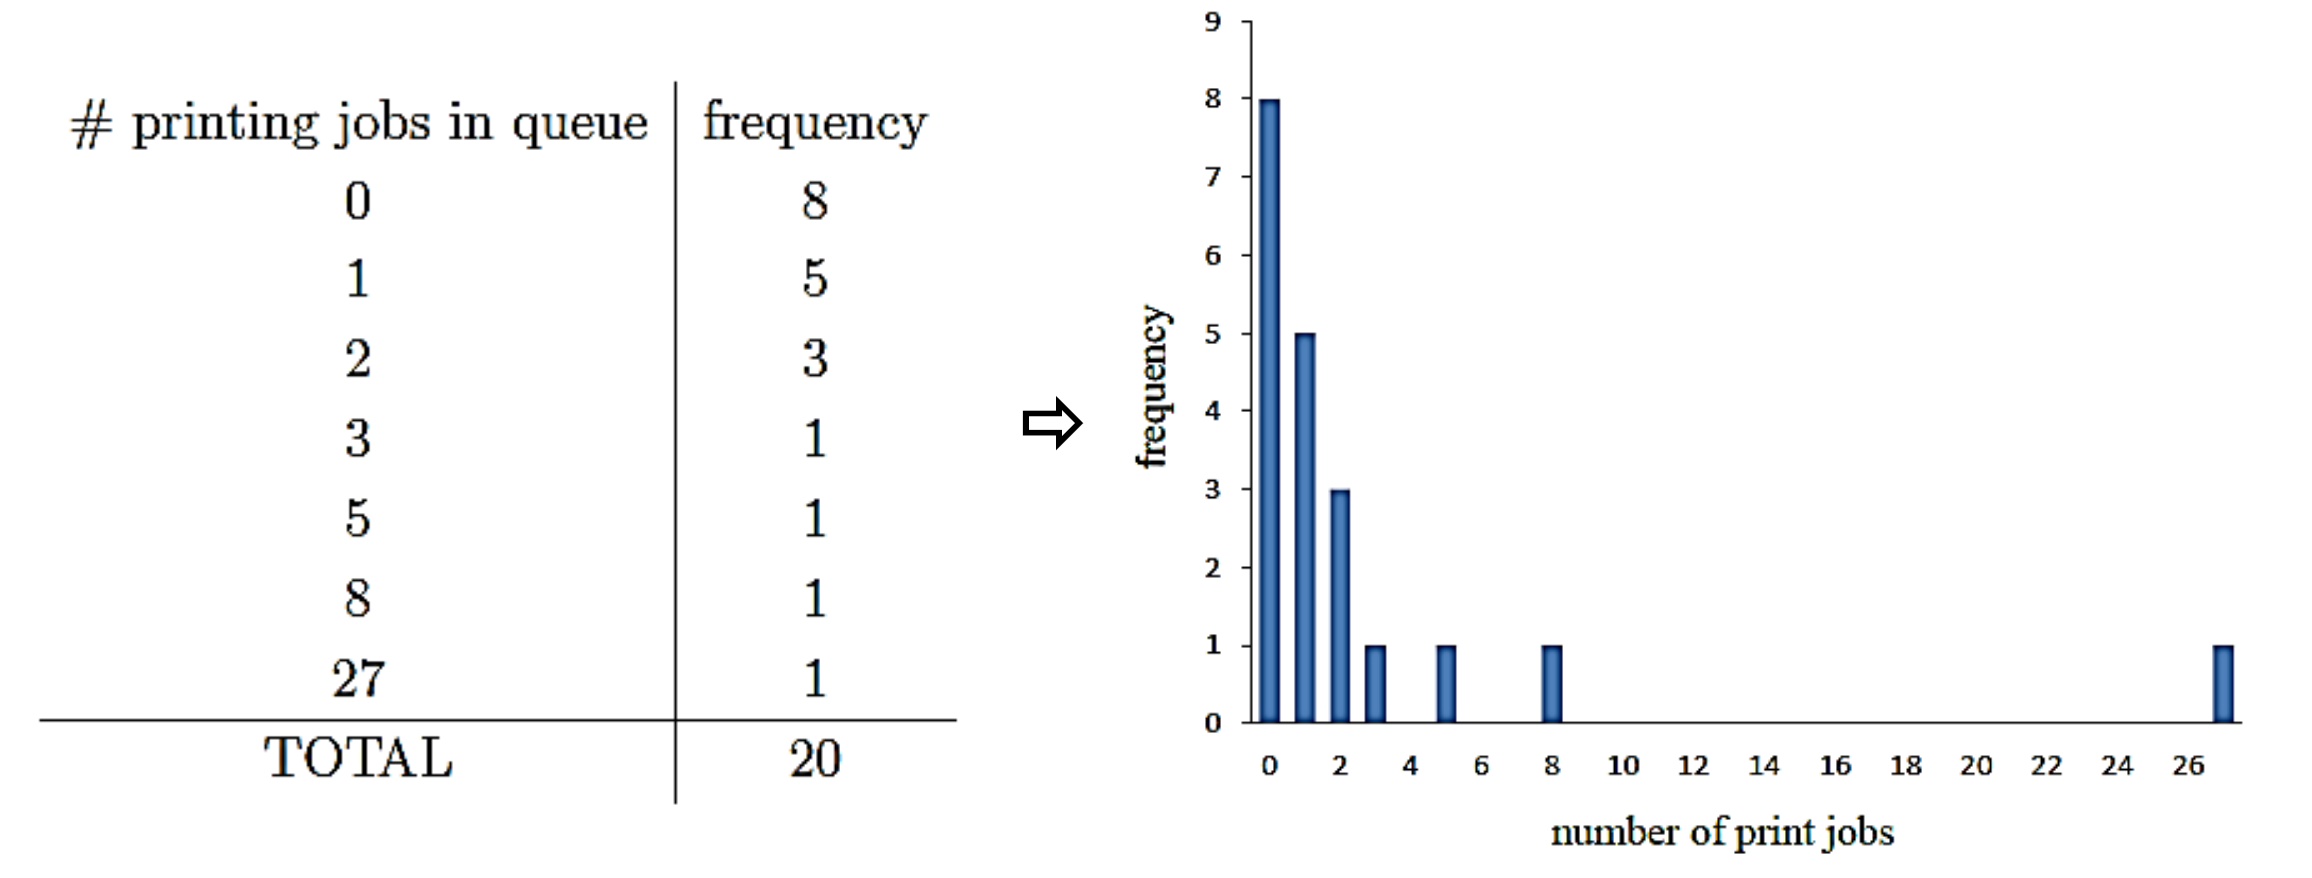
\includegraphics
            [width=0.5\textwidth]
            {content/img/1-bar-chart.png}
        \caption{Bar chart.}
        \label{fig:bar-chart-example}
    \end{figure}
    
    \begin{itemize}
        \item \textit{Height} of each bar $\propto$ \textit{frequency} of the value
        \item Can also use \textit{relative frequencies} (proportions) instead
    \end{itemize}
\end{definition}

\begin{definition}[Histogram]
    Suitable for \textit{continuous} data.
    
    The data range can be \textit{partitioned} into \textit{class intervals}.
    
    \begin{figure}[H]
        \centering
        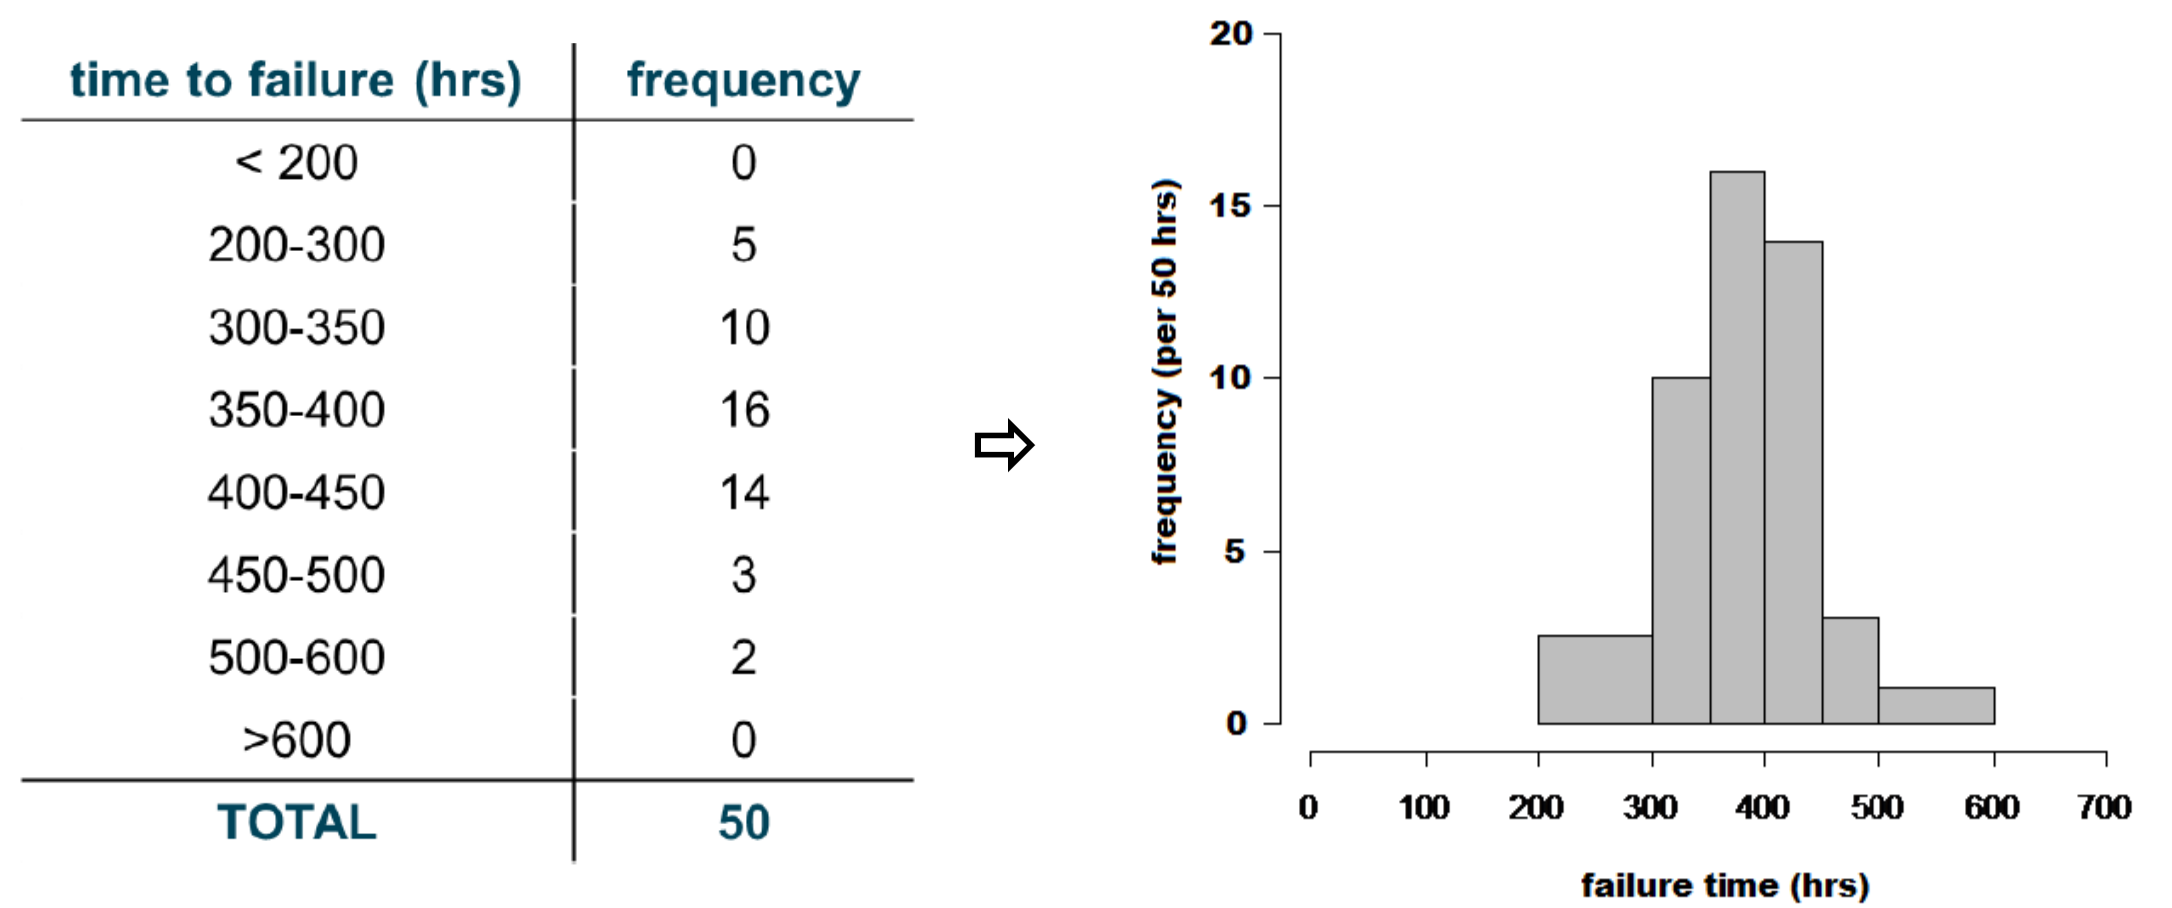
\includegraphics
            [width=0.5\textwidth]
            {content/img/1-histogram.png}
        \caption{Histogram.}
        \label{fig:histogram-example}
    \end{figure}

    \begin{itemize}
        \item \textit{Area} of each box $\propto$ \textit{frequency} of the class interval.
        \item Can also use the \textit{relative frequencies} (proportions) instead.
    \end{itemize}
\end{definition}

\subsection{Summary Statistics}

We can calculate \textit{summative measures} from data.

\begin{definition}[Summative Measures]\
    \begin{itemize}
        \item Measures of \textbf{location}:
        \begin{enumerate}
            \item Mean
            \item Median
            \item Mode
        \end{enumerate}
        \item Measures of \textbf{dispersion}:
        \begin{enumerate}
            \item Sample variance $s^2$ (and sample standard deviation $s$)
            \item Range
            \item Interquartile range
            \item Coefficient of variation
        \end{enumerate}
    \end{itemize}
\end{definition}

\begin{definition}[Mean]
    One type of \textit{average}.
    
    Given $n$ \textit{observations}, each denoted as $x_i$, then the sample mean $\Bar{x}$ is defined by
    
    \begin{equation}\label{eq:mean}
        \Bar{x} = \frac{1}{n} \sum \limits_{i=1}^{n} x_i
    \end{equation}
    
    Given $n$ \textit{observed values}, with each observed value $x_i$ observed $f_i$ times (frequency $f_i$), then the sample mean $\Bar{x}$ is defined by
    
    \begin{equation}\label{eq:mean_freq}
        \Bar{x} = \frac{
            \sum \limits_{i=1}^{n} f_i x_i
        }{
            \sum \limits_{i=1}^{n} f_i
        }
    \end{equation}
\end{definition}

\begin{definition}[Median]
    The \textit{median} is the \enquote{\textit{middle}} value.
    
    \begin{itemize}
        \item If the number of values $n$ is \textit{odd}, then the median $m$ is the value:
        \begin{equation}
            m = x_{\Ceil{\frac{n}{2}}}
        \end{equation}
        \item If the number of values $n$ is \textit{even}, then the median $m$ is the mean of the center two values:
        \begin{equation}
            m = \frac{
                x_{\frac{n}{2}} +
                x_{\frac{n}{2} + 1}
            }{2}
        \end{equation}
    \end{itemize}
    
    The median is a better \enquote{average} measure than the mean if the distribution is more \textit{skewed} (i.e. more values lie at the extremes).
\end{definition}

\begin{definition}[Mode]
    The \textit{mode} is the value which occurs most often (peak of distribution).
\end{definition}

\begin{definition}[Sample Variance]
    Given $n$ observations, each denoted $x_i$, then the \textit{sample variance} $s^2$ is computed by
    
    \begin{align}
        s^2 &= \frac{1}{n-1} \sum \limits_{i=1}^{n} \left(x_i - \Bar{x}\right)^2 \\
        &= \frac{1}{n-1} \left( \sum \limits_{i=1}^{n} x^2_i - n\Bar{x}^2 \right)
    \end{align}
    
    If given $N$ observed values with each value $x_i$ observed $f_i$ times (frequency $f_i$), then the \textit{sample variance} is also given by
    
    \begin{align}
        s^2 &= \frac{1}{n-1} \sum \limits_{i=1}^{N} f_i \left( x_i - \Bar{x} \right)^2 \\
        &= \frac{1}{n-1} \left( \sum \limits_{i=1}^{N} f_i x_i^2 - n \Bar{x}^2 \right)
    \end{align}

    Where the sample size $n$ is given by
    \begin{equation}
        n = \sum \limits_{i=1}^{N} f_i
    \end{equation}
\end{definition}

\begin{remark}
    For the sample variance the denominator is $n - 1$ because there is $n - 1$ \textit{degrees of freedom} within the sample. If we know the values of $n - 1$ samples and the sample mean $\Bar{x}$, then we can derive the last value.
\end{remark}

\begin{definition}[Sample Standard Deviation]
    The \textit{sample standard deviation} $s$ is simply the square root of the sample variance:
    
    \begin{equation}
        s = \sqrt{s^2}
    \end{equation}
\end{definition}

\begin{definition}[Range]
    The \textit{range} $r$ is the difference between the smallest value $x_\text{min}$ and largest value $x_\text{max}$
    
    \begin{equation}
        r = x_\text{max} - x_\text{min}
    \end{equation}
\end{definition}

\begin{definition}[Interquartile Range]
    The \textit{interquartile range} $i$ is the range of the \enquote{\textit{middle half}} of the data.
    
    The data is divided into four quartiles:
    \begin{enumerate}
        \item Lower quartile $Q_1$
        \item Median $Q_2$
        \item Upper quartile $Q_3$
    \end{enumerate}
    
    \begin{equation}
        i = Q_3 - Q_1
    \end{equation}
    
    It is less sensitive to the extreme observations within the data.
\end{definition}

\begin{definition}[Coefficient of Variation]
    The \textit{coefficient of variation} $CV$ is given by
    
    \begin{equation}
        CV = \frac{s}{\Bar{x}}
    \end{equation}
    
    It measures the \textit{spread} of the data relative to its mean (for positive data).
\end{definition}

\subsection{Sample vs Population}

\begin{definition}[Sample Statistic vs Population Statistic]
    The \textit{sample mean} $\Bar{x}$ is an \textit{estimate} for the \textit{population mean} $\mu$
    
    \begin{equation}
        \Bar{x}
        \xRightarrow{\text{estimates}}
        \mu
    \end{equation}
    
    The same holds for the sample / population median, the sample / population variance, etc.
\end{definition}
